\documentclass[10pt]{beamer}
%%%%%%%%%%%%%%%%%%%%%%%%%%%%%%%%%%%%%%%%%%%%%%%%%%%%%%%%%%%
%%%%% 	French, accents and font coding     	      %%%%%
%%%%%%%%%%%%%%%%%%%%%%%%%%%%%%%%%%%%%%%%%%%%%%%%%%%%%%%%%%%

\usepackage[french]{babel}
%\usepackage{enumitem} 
\usepackage{fancyhdr}
\usepackage[utf8]{inputenc}
\usepackage{bbm, amsmath, amssymb, amsthm, amsfonts}			% for theorem definitions


\usepackage{graphicx}			% for images and graphics
\usepackage{stmaryrd}			% for \llbracket symbols [[ ]]

%%%%%%%%%%%%%%%%%%%%%%%%%%%%%%%%%%%%%%%%%%%%%%%%%%%%%%%%%%%
%%%%%  		 Theorems etc.                        %%%%%
%%%%%%%%%%%%%%%%%%%%%%%%%%%%%%%%%%%%%%%%%%%%%%%%%%%%%%%%%%%

\newtheorem{Thm}{Théorème}[section]
\newtheorem{Cor}{Corolaire}[Thm]
\newtheorem{Prop}{Proposition}[section]
\newtheorem{Lem}{Lemme}[section]
\theoremstyle{definition}
\newtheorem{Def}{Définition}[section]
\newtheorem{Ex}{Exemple}[section]
\newtheorem{Exo}{Exercice}[section]
\theoremstyle{remark}
\newtheorem*{Rque}{Remarque}
\theoremstyle{definition}
\newtheorem{Algo}{Algorithme}[section]

%%%%%%%%%%%%%%%%%%%%%%%%%%%%%%%%%%%%%%%%%%%%%%%%%%%%%%%%%%%
%%%%%  		Hyperlinks                            %%%%%
%%%%%%%%%%%%%%%%%%%%%%%%%%%%%%%%%%%%%%%%%%%%%%%%%%%%%%%%%%%
\usepackage{hyperref}
\hypersetup{
    colorlinks=true,
    linkcolor=blue,
    filecolor=magenta,      
    urlcolor=cyan,
}
%%%%%%%%%%%%%%%%%%%%%%%%%%%%%%%%%%%%%%%%%%%%%%%%%%%%%%%%%
%%%%		For Algorithms
%%%%
%%%%%%%%%%%%%%%%%%%%%%%%%%%%%%%%%%%%%%%%%%%%%%%%%%%%%%%%%
\usepackage[ruled, vlined, french, onelanguage, algosection, nofillcomment, scleft]{algorithm2e}
\SetKwBlock{KwInit}{Initialization :}{endInit}


%%%%%%%%%%%%%%%%%%%%%%%%%%%%%%%%%%%%%%%%%%%%%%%%%%%%%%%%%%%
%%%%%  		Code			 %%%%%
%%%%%%%%%%%%%%%%%%%%%%%%%%%%%%%%%%%%%%%%%%%%%%%%%%%%%%%%%%%
\usepackage[section]{minted}
\usemintedstyle{borland}
\usepackage{color}
\definecolor{bg}{rgb}{0.95,0.95,0.95}

%%%%%%%%%%%%%%%%%%%%%%%%%%%%%%%%%%%%%%%%%%%%%%%%%%%%%%%%%
%%%%%		table of contents						%%%%%
%%%%%%%%%%%%%%%%%%%%%%%%%%%%%%%%%%%%%%%%%%%%%%%%%%%%%%%%%
\AtBeginSection{
	\begin{frame}
		\tableofcontents[currentsection, hideothersubsections]
	\end{frame}
}

%%%%%%%%%%%%%%%%%%%%%%%%%%%%%%%%%%%%%%%%%%%%%%%%%%%%%%%%%%%
%%%%%  		 latin abbreviations                  %%%%%
%%%%%%%%%%%%%%%%%%%%%%%%%%%%%%%%%%%%%%%%%%%%%%%%%%%%%%%%%%%
\newcommand{\ie}{{\em i.e.,~}}
\newcommand{\eg}{{\em e.g.,~}}
\newcommand{\lcf}{{\em cf.~}}



%%%%%%%%%%%%%%%%%%%%%%%%%%%%%%%%%%%%%%%%%%%%%%%%%%%%%%%%%%%
%%%%%  		 Style math                         %%%%%
%%%%%%%%%%%%%%%%%%%%%%%%%%%%%%%%%%%%%%%%%%%%%%%%%%%%%%%%%%%

\newcommand{\nset}{\mathbb{N}}
\newcommand{\zset}{\mathbb{Z}}
\newcommand{\rset}{\mathbb{R}}
\newcommand{\cset}{\mathbb{C}}
\newcommand{\qset}{\mathbb{Q}}
\newcommand{\kset}{\mathbb{K}}
\newcommand{\tset}{\mathbb{T}}
\newcommand{\xset}{\mathbb{X}}
\newcommand{\yset}{\mathbb{Y}}
\newcommand{\uset}{\mathbb{U}}
\newcommand{\fset}{\mathbb{F}}
\newcommand{\mset}{\mathbb{M}}

\newcommand{\ps}{\text{ p.s. }}
\newcommand{\geqrespleq}{\underset{\mbox{ (resp $\leq$) }}{\geq}}
\newcommand{\leqrespgeq}{\underset{\mbox{ (resp $\geq$) }}{\leq}}



\usepackage{xifthen}
%\newcommand{\EE}[1][]{%
%  \ifthenelse{\isempty{#1}}%
%    {\mathbb{E}}% if #1 is empty
%    {\mathbb{E}\left[#1\right]}% if #1 is not empty
%}

%\newcommand{\PP}[1][]{%
%  \ifthenelse{\isempty{#1}}%
%    {\mathbb{P}}% if #1 is empty
%    {\mathbb{P}\left(#1\right)}% if #1 is not empty
%}

\newcommand{\law}[1][]{%
  \ifthenelse{\isempty{#1}}%
    {\calL}% if #1 is empty
    {\calL \left(#1\right)}% if #1 is not empty
}

%\newcommand{\pp}[1][]{%
%  \ifthenelse{\isempty{#1}}%
%    {p}% if #1 is empty
%    {p\left(#1\right)}% if #1 is not empty
%}
% 
%\newcommand{\Cov}[1][]{%
%  \ifthenelse{\isempty{#1}}%
%    {\mathrm{Cov}}% if #1 is empty
%    {\mathrm{Cov}\left(#1\right)}% if #1 is not empty
%}
% 
%\newcommand{\Var}[1][]{%
%  \ifthenelse{\isempty{#1}}%
%    {\mathrm{Var}}% if #1 is empty
%    {\mathrm{Var}\left(#1\right)}% if #1 is not empty
%  }

\usepackage{xparse}
\DeclareDocumentCommand{\PP}{go}
{\IfNoValueTF{#2}
  {\IfNoValueTF{#1}
    {\mathbb{P}}
    {\mathbb{P}_{#1}}%
  }
  {\IfNoValueTF{#1}
    {\mathbb{P}\left(#2\right)}
    {\mathbb{P}_{#1}\left(#2\right)}%
  }%
}

\DeclareDocumentCommand{\EE}{go}
{\IfNoValueTF{#2}
  {\IfNoValueTF{#1}
    {\mathbb{E}}
    {\mathbb{E}_{#1}}%
  }
  {\IfNoValueTF{#1}
    {\mathbb{E}\left[#2\right]}
    {\mathbb{E}_{#1}\left[#2\right]}%
  }%
}

\DeclareDocumentCommand{\pp}{go}
{\IfNoValueTF{#2}
  {\IfNoValueTF{#1}
    {p}
    {p_{#1}}%
  }
  {\IfNoValueTF{#1}
    {p\left(#2\right)}
    {p_{#1}\left(#2\right)}%
  }%
}

\DeclareDocumentCommand{\Cov}{go}
{\IfNoValueTF{#2}
  {\IfNoValueTF{#1}
    {\mathrm{Cov}}
    {\mathrm{Cov}_{#1}}%
  }
  {\IfNoValueTF{#1}
    {\mathrm{Cov}\left(#2\right)}
    {\mathrm{Cov}_{#1}\left(#2\right)}%
  }%
}

\DeclareDocumentCommand{\Var}{go}
{\IfNoValueTF{#2}
  {\IfNoValueTF{#1}
    {\mathrm{Var}}
    {\mathrm{Var}_{#1}}%
  }
  {\IfNoValueTF{#1}
    {\mathrm{Var}\left(#2\right)}
    {\mathrm{Var}_{#1}\left(#2\right)}%
  }%
}



\def\1{\mathbf 1}
\def\ind{\mathbbm 1}
\newcommand{\mb}{\mathbf}
\newcommand{\ud}{\,\mathrm{d}} 
\newcommand{\given}[1][{}]{\;\middle\vert\;{#1} }
\def\indep{\perp\!\!\!\perp}


%%%%%%%%%%%%%%%%%%%%%%%%%%%%%%%%%%%%%%%%%%%%%%%%%%%%%%%%%%%
%%%%%        equality symbols                        %%%%%
%%%%%%%%%%%%%%%%%%%%%%%%%%%%%%%%%%%%%%%%%%%%%%%%%%%%%%%%%%%
\newcommand{\deq}{\stackrel{\rm def}{=}}
\newcommand{\eqlaw}{\stackrel{\rm loi}{=}}
\newcommand{\siid}{\stackrel{\rm iid}{\sim}}
\newcommand{\cps}{\xrightarrow[n \to +\infty]{\ps}}
\newcommand{\cprob}{\xrightarrow[n \to +\infty]{P}}
\newcommand{\claw}{\xrightarrow[n \to +\infty]{\calL}}


%%%%%%%%%%%%%%%%%%%%%%%%%%%%%%%%%%%%%%%%%%%%%%%%%%%%%%%%%%%
%%%%%        maths symbols                    	     %%%%%
%%%%%%%%%%%%%%%%%%%%%%%%%%%%%%%%%%%%%%%%%%%%%%%%%%%%%%%%%%%
\usepackage{amsopn}
\DeclareMathOperator{\ch}{ch}
\DeclareMathOperator{\sh}{sh}
\DeclareMathOperator{\argch}{argch}
\DeclareMathOperator{\argsh}{argsh}
\DeclareMathOperator{\argth}{argth}

\DeclareMathOperator{\sign}{sign}
\DeclareMathOperator{\Card}{Card}
\DeclareMathOperator{\rg}{rg}
\DeclareMathOperator{\tr}{tr}

\DeclareMathOperator{\corr}{corr}
\DeclareMathOperator{\var}{var}
\DeclareMathOperator{\vect}{vect}

\DeclareMathOperator{\cov}{cov}
\DeclareMathOperator{\pred}{pred}
\DeclareMathOperator{\Id}{Id}

\renewcommand{\Re}{\mathop{\mathrm{Re}}}
\newcommand{\argmin}{\mathop{\mathrm{arg\,min}}}
\newcommand{\argmax}{\mathop{\mathrm{arg\,max}}}
\newcommand{\spn}{\mathop{\mathrm{span}}}
\def\rang{\mathop{\rm rang}\nolimits}
\def\Ker{\mathop{\rm Ker}\nolimits}
\def\Im{\mathop{\rm Im}\nolimits}
\def\Vect{\mathop{\rm Vect}\nolimits}
\def\proj{\mathop{\rm proj}\nolimits}




\def\dim{\mathop{\rm dim}\nolimits}

\def\dom{\mathop{\rm dom}\nolimits}
\def\supp{\mathop{\rm supp}\nolimits}
\def\relint{\mathop{\rm relint}\nolimits}
\def\prox{\mathop{\rm prox}\nolimits}

\def\bfr{\mathbf{r}}
\def\bfx{\mathbf{x}}
\def\bfX{\mathbf{X}}

\def\bfy{\mathbf{y}}
\def\bftheta{\boldsymbol{\theta}}


\def\calA{\mathcal{A}}
\def\calB{\mathcal{B}}
\def\calC{\mathcal{C}}
\def\calD{\mathcal{D}}
\def\calE{\mathcal{E}}
\def\calF{\mathcal{F}}
\def\calG{\mathcal{G}}
\def\calH{\mathcal{H}}
\def\calI{\mathcal{I}}
\def\calJ{\mathcal{J}}
\def\calK{\mathcal{K}}
\def\calL{\mathcal{L}}
\def\calM{\mathcal{M}}
\def\calN{\mathcal{N}}
\def\calO{\mathcal{O}}
\def\calP{\mathcal{P}}
\def\calQ{\mathcal{Q}}
\def\calR{\mathcal{R}}
\def\calS{\mathcal{S}}
\def\calT{\mathcal{T}}
\def\calU{\mathcal{U}}
\def\calV{\mathcal{V}}
\def\calW{\mathcal{W}}
\def\calX{\mathcal{X}}
\def\calY{\mathcal{Y}}
\def\calZ{\mathcal{Z}}

\def\cH{\calH}
\def\cN{\calN}


\newcommand{\tnorm}[1]{{\left\vert\kern-0.25ex\left\vert\kern-0.25ex\left\vert #1 
    \right\vert\kern-0.25ex\right\vert\kern-0.25ex\right\vert}} % triple norm

\newcommand{\inner}[1]{{
\left\langle #1 \right\rangle}} % inner product

\newcommand{\norm}[1]{{
\left\| #1 \right\|}} % norm

\newcommand{\abs}[1]{{
\left| #1 \right|}} % abs

\newcommand{\piecewise}[1]{{
    \left\lbrace \begin{array}{ll} #1 \end{array} \right. }} % for piecewise functions

\newcommand{\fundef}[1]{{
\begin{array}{lcl} #1 \end{array} }} % for functions definitions

\newcommand{\seg}[1]{{\left[ #1 \right]}} % closed segment [ ]
\newcommand{\osego}[1]{{\left] #1 \right[}} % open segment ] [
\newcommand{\oseg}[1]{{\left] #1 \right]}} % semi-open segment ] ]
\newcommand{\sego}[1]{{\left[ #1 \right[}} % semi-open segment [ [
\newcommand{\iseg}[1]{{\left\llbracket #1 \right\rrbracket}} % integer segment

\newcommand{\ens}[1]{{
\left\lbrace #1 \right\rbrace }} % ensemble

\newcommand{\floor}[1]{{
\left\lfloor #1 \right\rfloor }} % floor

\newcommand{\pivot}[3]{{
    \left(
      \begin{array}{#1|#2}
        #3
      \end{array}
    \right)
  }}
\usepackage{color}
\newcommand{\red}{\color{red}}
\definecolor{gray}{rgb}{0.4, 0.4, 0.4}
\usepackage{sansmathaccent}
\pdfmapfile{+sansmathaccent.map}
\usepackage{movie15}
\setbeamertemplate{footline}[frame number]
\title[HMC]{Introduction aux méthodes de Monte Carlo par dynamique Hamiltonienne}
\author{Shmuel RAKOTONIRINA-RICQUEBOURG, Amaury DURAND}

\begin{document}
\begin{frame}
\titlepage
\end{frame}
\begin{frame}
  \frametitle{Plan}
  \tableofcontents[hideallsubsections]
\end{frame}

\section{Introduction}

\subsection{Algorithmes MCMC}

\begin{frame}
	\frametitle{Principe des MCMC}
	\begin{itemize}
		\item Objectif : pour $\pi$ à densité $h_\pi$ simuler $\pi$ ou approcher $\pi f$
		\item Idée : trouver une chaîne de Markov $X$ admettant $\pi$ comme loi invariante et convergeant vers $\pi$
	\end{itemize}
	\begin{Thm}[Théorème ergodique]\label{thm:ergodic}
		Soit $(X_k)_{k \in \nset}$ une chaîne de Markov de noyau $P$ sur $(\xset, \calX)$ admettant une unique loi invariante $\pi$. Alors pour tout $f \in \fset_+(\xset, \calX) \cup \fset_b(\xset, \calX)$ et pour $\pi$-presque tout $x \in \xset$,
		$$\frac{1}{n} \sum_{k=0}^{n-1} f(X_k) \xrightarrow[n \to +\infty]{\PP_x\text{-}\ps} \pi f$$
	\end{Thm}
\end{frame}

\subsection{Algorithme de Metropolis (Random Walk Metropolis)}

\begin{frame}
  \frametitle{Algorithme Random-walk Metropolis}
  \begin{center}
    {\small 
		\begin{algorithm}[H]
			\KwData{$h_\pi$ proportionnel à la densité cible, $Q$ loi simulable}
			$X_0 \leftarrow x \in \xset$ arbitraire\;
			$(U_k)_{k \in \nset} \siid Q$ \;
			\Repeat{une condition d'arrêt}{
				$Y_{k+1} \leftarrow X_k + U_{k+1}$ \tcp*{Proposer un mouvement}
				$\alpha_{k+1} \leftarrow \alpha(X_k, Y_{k+1})$ où $\alpha(x,y) = 1 \wedge \frac{h_{\pi}(y)}{h_\pi(x)}$\;
				$X_{k+1} \leftarrow \piecewise{ Y_{k+1} & \text{avec probabilité } \alpha_{k+1} \\ X_k & \text{avec probabilité } 1 - \alpha_{k+1}}$ \tcp*{Accepter ou rejeter}
			}
			\KwRet{$(X_k)_k$}
			\caption{Random Walk Metropolis}
			\label{algo:metropolis}
                      \end{algorithm}
                      }
	\end{center}
\end{frame}

\section{Dynamique hamiltonienne}

\subsection{Définition}

\begin{frame}
	\frametitle{Dynamique hamiltonienne}
	\begin{Def}(Dynamique hamiltonienne)
		Soit $H : \fundef{\rset^d \times \rset^d & \to & \rset \\ (x,p) & \mapsto & H(x,p)}$. Deux fonctions de position $x : \rset_+ \to \rset^d$ et de quantité de mouvement $p : \rset_+ \to \rset^d$ sont dites solutions du hamiltonien $H$ (ou suivant la dynamique hamiltonienne de $H$) si
		\begin{equation*}\label{eq:hamiltonian-dyn}
			\begin{aligned}
				x'(t) &= \frac{\partial H}{\partial p} (x(t), p(t)) \\
				p' (t) &= -\frac{\partial H}{\partial x} (x(t), p(t))
			\end{aligned}
		\end{equation*}
	\end{Def}
	Pour $T>0$, $H$ peut être associée à la densité (sur $\rset^{2d}$)
	$$
	h(z) \propto \exp \left( -\frac{H(z)}{T} \right)
	$$
\end{frame}
 
\begin{frame}
	\frametitle{Hamiltonien pour l'algorithme HMC}
	Pour avoir $X \sim \pi$, on cherche à simuler $(X,P) \sim \widetilde \pi = \pi \otimes \nu$ pour une loi $\nu$ choisie. Dans toute la suite, on fera les hypothèses suivantes :
	\begin{Hyp}[H]\label{hyp:hyp}
		\begin{itemize}
			\item $\pi$ et $\nu$ sont à densité $h_\pi$ et $h_\nu$ strictement positives sur $\rset^d$
			\item $\exists k \geq 1, \ln(h_\pi)$ et $\ln(h_\nu)$ sont de classe $\calC^k$ sur $\rset^d$
			\item $h_\nu$ est paire
			\item $H : (x,p) \mapsto U(x) + K(p)$ avec $U = - T \ln(h_\pi), K = -T \ln(h_\nu)$
		\end{itemize}
	\end{Hyp}
	Ainsi, la densité $h \propto e^{H/T}$ est la densité jointe $h = h_\pi \otimes h_\nu = h_{\widetilde \pi}$.
\end{frame}
 
\subsection{Propriétés}

\begin{frame}
	\frametitle{Flot de l'équation différentielle}
	En notant $z = (x,p)$, les équations $x' = \frac{\partial H}{\partial p}, p' = -\frac{\partial H}{\partial x}$ se réécrivent $z' = F(z)$ où $F = J \nabla H$ et
	$J = \begin{bmatrix}
		0_{d} & I_{d} \\
		-I_{d} & 0_{d}
              \end{bmatrix}$.
              \begin{Def}[flot hamiltonien]
		Pour $t \in \rset$, on définit le flot $\phi_t$ de sorte que pour tout $z_0 \in \rset^{2d}$, $t \mapsto \phi_t(z_0)$ soit l'unique solution du hamiltonien avec condition initiale $z(0) = z_0$.
              \end{Def}
\end{frame}
\begin{frame}            
  \frametitle{Propriétés des solutions}
  	\begin{Prop}[conservation du hamiltonien]
		Le hamiltonien est conservé le long des trajectoires : si $z' = F(z)$, alors $H \circ z$ est constant.
	\end{Prop}
	
	\begin{Prop}[conservation du volume]
		La solution du hamiltonien conserve le volume : $\detjacob{\phi_t}{z} = 1$.
	\end{Prop}
\end{frame}

\begin{frame}
	\frametitle{Réversibilité du flot}
	\begin{Lem}[réversibilité du temps]
		Soit $z = (x,p)$ une solution du hamiltonien $H$. On définit $\bar{z} = (\bar x, \bar p)$ par $\bar z(t) = (x(-t), -p(-t))$. Alors
		\begin{enumerate}
			\item $\bar{z}$ est solution du hamiltonien $H$ (avec d'autres conditions initiales).
			\item $\forall t \in \rset_+, \phi_t(\bar{z}(-t)) = \bar{z}(0)$
		\end{enumerate}
	\end{Lem}
	\begin{Prop}[réversibilité du flot]
		$\phi_t$ est un $\calC^k$-difféomorphisme d'inverse $\phi_t^{-1}  = s \circ \phi_t \circ s : (x,p) \mapsto (\phi_t^{(1)}(x, -p), - \phi_t^{(2)}(x, -p))$ avec $s : (x,p) \mapsto (x,-p)$. 
	\end{Prop}
\end{frame}

\begin{frame}
  \frametitle{Preuve de la réversibilité du temps}
		Par définition, $\bar{z}(t) = s \circ z (-t)$ et par hypothèse de parité de $h_\nu$, $H = H \circ s$.

		Notons $S \doteq \frac{ds}{dz}(z) = \begin{bmatrix} I_d & 0_d \\ 0_d & -I_d \end{bmatrix}$ (et ce pour tout $z$). Ainsi, $\nabla H = S \nabla H \circ s$. On remarque que $SJ = -JS$ et $s^{-1} = s$.

		$$\bar z'(t) = -Sz'(-t) = -SJ\nabla H(z(-t)) = JS \nabla H(z(-t))$$
		donc
		$$\bar z'(t) = J \nabla H (s^{-1}(z(-t))) = J \nabla H(\bar z(t))$$
                \null\hfill\qedsymbol
\end{frame}

\begin{frame}
  \frametitle{Preuve de la réversibilité du flot}
		Il suffit de prouver la formule de l'inverse. On pose $\bar \phi_t = s \circ \phi_t \circ s$. On fixe $z_0 = (x_0,p_0)$ et on note $z$ la solution du hamiltonien avec $z(0) = z_0$.
		\begin{itemize}
			\item D'une part,
			$$
			\bar \phi_t(\phi_t(x_0,p_0)) = \bar \phi_t(z(t)) = (\phi_t^{(1)}(\bar z(-t)), - \phi_t^{(2)}(\bar z(-t))) = (x_0, p_0)
			$$
			car $\bar z(0) = (x_0,-p_0)$.

			\item D'autre part,
			$$
			\bar \phi_t(x_0,-p_0) = (\phi_t^{(1)}(x_0, p_0), - \phi_t^{(2)}(x_0, p_0)) = (x(t),-p(t)) = \bar z(-t)
			$$
			donc
			$$
			\phi_t (\bar \phi_t(x_0,-p_0)) = \phi_t(\bar z(-t)) = \bar{z}(0) = (x_0,-p_0).
			$$
                      \end{itemize}
                      \null\hfill\qedsymbol
\end{frame}
 
\subsection{Discrétisation}

\begin{frame}
	\frametitle{Algorithme du leapfrog}
	Variante de la méthode d'Euler : on discrétise $x' = \nabla K(p), p' = - \nabla U(x)$ en
	\begin{enumerate}
		\item $p_{t+\epsilon/2} = p_t - \frac{\epsilon}{2} \nabla U(x_t)$ (demi-pas en $p$).
		\item $x_{t+\epsilon} = p_t + \epsilon \nabla K(p_{t+\epsilon/2})$ (pas en $x$).
		\item $p_{t+\epsilon} = p_{t+\epsilon/2} - \frac{\epsilon}{2} \nabla U(x_{t+\epsilon})$ (demi-pas en $p$).
	\end{enumerate}
	\begin{center}
		\begin{algorithm}[H]
			\KwData{pas $\epsilon$, nombre de pas $L$, état initial $(x_0,p_0)$}
			\For(\tcp*[h]{Saute-mouton}){$k \in \iseg{0, L-1}$}{
				$x_{k+1} \leftarrow x_k + \epsilon \nabla K \left( p_k - \frac{\epsilon}{2} \nabla U(x_k) \right)$\;
				$p_{k+1} \leftarrow p_k - \frac{\epsilon}{2} \nabla U(x_k) - \frac{\epsilon}{2} \nabla U(x_{k+1})$\;
			}
			\KwRet{$(x_L,p_L)$}
			\caption{Discrétisation de l'évolution par saute-mouton ({\it leapfrog})}
			\label{algo:leapfrog}
		\end{algorithm}
	\end{center}
\end{frame}

\begin{frame}
	\frametitle{Flot approché}
	\begin{center} % je rappelle l'algorithme pour que le public voit d'où sort la déf
		\small
		\begin{algorithm}[H]
			\KwData{pas $\epsilon$, nombre de pas $L$, état initial $(x_0,p_0)$}
			\For(\tcp*[h]{Saute-mouton}){$k \in \iseg{0, L-1}$}{
				$x_{k+1} \leftarrow x_k + \epsilon \nabla K \left( p_k - \frac{\epsilon}{2} \nabla U(x_k) \right)$\;
				$p_{k+1} \leftarrow p_k - \frac{\epsilon}{2} \nabla U(x_k) - \frac{\epsilon}{2} \nabla U(x_{k+1})$\;
			}
			\KwRet{$(x_L,p_L)$}
                        \caption{Discrétisation de l'évolution par saute-mouton ({\it leapfrog})}
		\end{algorithm}
	\end{center}
	\begin{Def}[flot approché] \label{def:flot_approche}
		On fixe $\epsilon > 0$. Pour $L \in \nset^*$, on définit le flot approché du hamiltonien par $L$ itérations de l'algorithme leapfrog par $\hat{\phi}_L = \hat{\phi}^L$ où $\hat \phi$ est défini par
		\begin{align*}
		\hat{\phi}^{(1)} : (x,p) & \mapsto x + \epsilon \nabla K \left( p - \frac{\epsilon}{2} \nabla U(x) \right) \\
		\hat{\phi}^{(2)} : (x,p) & \mapsto p - \frac{\epsilon}{2} \nabla U(x) - \frac{\epsilon}{2} \nabla U(\hat{\phi}^{(1)}(x,p))
		\end{align*}
	\end{Def}
\end{frame}

\begin{frame}
	\frametitle{Propriétés du flot approché}
	\begin{Prop}[conservation du volume]
		On suppose $k \geq 2$ ($U$ et $K$ de classe $\calC^2$). La solution approchée du hamiltonien par le leapfrog conserve le volume : $\detjacob{\hat \phi}{z} = 1$.
	\end{Prop}
	\begin{Prop}[réversibilité du flot approché]
		$\hat \phi$ est inversible d'inverse $\phi^{-1} = s \circ \hat \phi \circ s : (x,p) \mapsto (\hat{\phi}^{(1)}(x,-p), -\hat{\phi}^{(2)}(x,-p))$.
	\end{Prop}
\end{frame}
 
\section{Hamiltonian Monte-Carlo}

\subsection{Cas idéal}
 
% invariance de la loi
 
\begin{frame}
	\frametitle{Algorithme HMC idéal}
	\begin{center}
		\begin{algorithm}[H]
			\KwData{$h_\pi$ proportionnel à la densité cible, $t$ une durée sur laquelle suivre la dynamique}
			$X_0 \leftarrow x \in \xset$ arbitraire\;
			\Repeat{une condition d'arrêt}{
				$\tilde{P}_k \sim \mathcal \nu$ et $\tilde{P}_k \indep (Z_0, \cdots, Z_{k})$ \tcp*{Tirer la quantité de mouvement}
				$\tilde{Z}_k \leftarrow (X_k, \tilde{P}_k)$ \;
				$Z_{k+1} = (X_{k+1}, P_{k+1}) \leftarrow \phi_t(\tilde{Z}_k)$ \tcp*{Suivre la dynamique}
			}
			\KwRet{$(X_k)_k$}
			\caption{Hamiltonian Monte-Carlo, cas idéal}
			\label{algo:HMC-ideal}
		\end{algorithm}
	\end{center}
\end{frame}

\begin{frame}
	\frametitle{Invariance de $\widetilde \pi$}
	\begin{Prop}
		Pour $t \in \rset_+$, le processus $(Z_k)_{k \in \nset}$ défini par l'algorithme \ref{algo:HMC-ideal} est une chaîne de Markov homogène de noyau $QR_t$ sur $\rset^{2d}$ avec
		$$
		Q((x,p),\cdot) = \delta_x \otimes \nu \text{ et } R_t((x,p),\cdot) = \delta_{\phi_t(z)}.
		$$
		De plus, $\widetilde{\pi}$ est $Q$ et $R_t$-invariante. 
	\end{Prop}
	{\bf Preuve de la $R_t$-invariance :}
		{\small
		\begin{align*}
		\widetilde{\pi} R_t (A)
		&= \int \widetilde{\pi}(dz) R_t(z, A)
		= c \int \exp \left(-\frac{H(z)}{T} \right) \ind_A(\phi_t(z)) dz\\
		&= c \int \exp \left(-\frac{H \circ \phi_t^{-1}(y)}{T} \right) \ind_A(y) dy
		= c \int \exp \left(-\frac{H(y)}{T} \right) \ind_A(y) dy \\
		&= \widetilde{\pi}(A).
		\end{align*}
                }
	\null\hfill\qedsymbol
\end{frame}
 
\subsection{Cas réel}
 
% réversibilité de la loi

\begin{frame}
	\frametitle{Modification du HMC pour la discrétisation}
	Contrairement à $\phi_t$, $\hat \phi_L$ ne conserve pas le hamiltonien.

	Idée : remplacer $\phi_t$ par $g \circ \hat \phi_L$ pour $g$ une fonction à déterminer, i.e. remplacer $R_t$ par
	$$
	\hat{R}_L : \fundef{
		\rset^{2d} \times \calB(\rset^{2d}) & \to & [0,1] \\
		(z, A) & \mapsto & \delta_{g \circ \hat{\phi}_L(z)}(A)
	}
	$$

	% Problème : $\widetilde \pi$ est $Q$-invariante mais pas $\hat R_L$-invariante.
        \pause
	\begin{Prop}[réversibilité]\label{prop:rever_discret}
		On suppose $k \geq 2$ ($U$ et $K$ de classe $\calC^2$). On prend $g = s$ et
		$$
		\alpha : (z_0,z_1) \mapsto 1 \wedge \frac{h_{\widetilde \pi}(z_1)}{h_{\widetilde \pi}(z_0)} = 1 \wedge \exp(\frac{-H(z_1)+H(z_0)}{T}).
		$$
		Si $\hat R_L^\alpha$ est le noyau de Metropolis-Hasting associé au noyau instrumental $\hat R_L$ et à la fonction de rejet $\alpha$, alors $\widetilde \pi$ est $\hat R_L^\alpha$-réversible (et donc $\hat R_L^\alpha$-invariant).
	\end{Prop}
\end{frame}

\begin{frame}
  \frametitle{Preuve de la réversibilité de la loi cible}
	
		\small
		Notons $\psi_L = s \circ \hat \phi_L$, de sorte que $\hat R_L(z,\cdot) = \delta_{\psi_L(z)}$. Ainsi,
		$$
		\hat R_L^\alpha(z,A) = \alpha(z,\psi_L(z)) \ind_A(\psi_L(z)) + (1-\alpha(z,\psi_L(z))) \ind_A(z)
		$$
		donc
		$$
		\widetilde \pi \otimes \hat R_L^\alpha (A \times B)
		=
		\Lambda_1(A,B) + \Lambda_2(A,B)
		$$
		où
		$$
		\Lambda_2(A,B) = \int \ind_A(z) \ind_B(z) (1-\alpha(z,\psi_L(z))) e^{-H(z)/T} dz \text{ est sym\'etrique}
		$$
		et
		$$
		\begin{aligned}
		\Lambda_1(A,B)
		&= \int \ind_A(z) \ind_B(\psi_L(z)) \alpha(z,\psi_L(z)) e^{-H(z)/T} dz\\
		&= \int \ind_A(z) \ind_B(\psi_L(z)) \left( e^{-H(z)/T} \wedge e^{-H(\psi_L(z))/T} \right) dz.
		\end{aligned}
		$$

		$\psi_L^{-1} = \psi_L$ (réversibilité de $\hat \phi_L$) et $\detjacob{\psi_L}{z} = -1$ (conservation du volume) donc le changement de variable $z \mapsto \psi_L(z)$ donne que $\Lambda_1$ est symétrique.
	\null\hfill\qedsymbol
\end{frame}
 
\begin{frame}
  \frametitle{Algorithme HMC réel}
        %\begin{center}
        %\small
	%        \begin{algorithm}[H]
	%        	\KwData{$h_\pi$ proportionnel à la densité cible, $\epsilon$ pas du saute-mouton, $L$ nombre de pas du saute-mouton}
	%        	$X_0 \leftarrow x \in \xset$ arbitraire\;
	%        	\Repeat{une condition d'arrêt}{
	%        		$P_k \sim \mathcal N(0,1)$\tcp*{Tirer la quantité de mouvement}
	%        		$(X_{prop},P_{prop}) \leftarrow \texttt{leapfrog}(X_k,P_k)$\tcp*{Proposer un mouvement}
	%        		$U_k \leftarrow U(X_k); K_k \leftarrow \norm{P_k}^2/2$\;
	%        		$U_{prop} \leftarrow U(X_{prop}); K_{prop} \leftarrow \norm{P_{prop}}^2/2$\;
	%        		\eIf{$\mathcal U([0,1]) < \exp(U_k-U_{prop}+K_k-K_{prop})$}{
	%        			$X_{k+1} \leftarrow X_{prop}$ \tcp*{Accepter}
	%        		}{
	%        			$X_{k+1} \leftarrow X_k$ \tcp*{Rejeter}
	%        		}
	%        	}
	%        	\KwRet{$(X_k)_k$}
	%        	\caption{Hamiltonian Monte-Carlo}
	%        	\label{algo:HMC}
	%        \end{algorithm}
        %      \end{center}
  \begin{center}
    {\small 
	\begin{algorithm}[H]
          \KwData{$h_\pi$ proportionnel à la densité cible, $\epsilon$ pas du saute-mouton, $L$ nombre de pas du saute-mouton}
          $X_0 \leftarrow x \in \xset$ arbitraire\;
          \Repeat{une condition d'arrêt}{
            $\tilde{P}_k \sim \mathcal \nu$ et $\tilde{P}_k \indep (Z_0, \cdots, Z_{k})$ \tcp*{\footnotesize  Tirer la quantité de mouvement}
            $\tilde{Z}_k \leftarrow (X_k, \tilde{P}_k)$ \;
            $Z_{k+1}^{\rm prop} = (X_{k+1}^{\rm prop}, P_{k+1}^{\rm prop}) \leftarrow s \circ \hat{\phi}_L(\tilde{Z}_k)$ \tcp*{ \footnotesize  Suivre la dynamique approchée} 
            $\alpha_{k+1} \leftarrow 1 \wedge \exp \left( \frac{- H(Z_{k+1}^{\rm prop}) + H(\tilde{Z}_k) }{T} \right)$ \;
            
            $Z_{k+1} \leftarrow \piecewise{ Z_{k+1}^{\rm prop} & \text{avec probabilité } \alpha_{k+1} \\ \tilde{Z}_k & \text{avec probabilité } 1 - \alpha_{k+1}}$ \tcp*{\footnotesize Accepter ou rejeter}
          }
          \KwRet{$(X_k)_k$}
          \caption{Hamiltonian Monte-Carlo, cas concret}
          \label{algo:HMC}
	\end{algorithm}
        }
\end{center}

\end{frame}
 
\section{Simulations}
\subsection{Loi normale}
\begin{frame}
  \frametitle{Loi normale : trajectoires}
\begin{center}
    \includemovie[autoplay, poster]{\textwidth}{.9\textheight}{figs/normal.mp4}
  \end{center}  
\end{frame}

\begin{frame}
  \frametitle{Loi normale : autocorrelations}
\begin{center}
      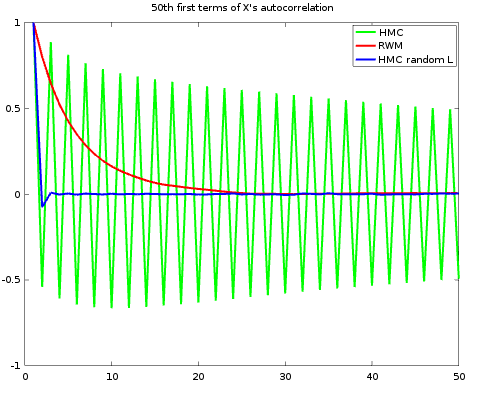
\includegraphics[width=.8\textwidth]{figs/normal_autocor.png}
  \end{center}  
\end{frame}

\begin{frame}
  \frametitle{Loi normale : loin du mode}
\begin{center}
    \includemovie[autoplay, poster]{\textwidth}{.9\textheight}{figs/normal_far.mp4}
  \end{center}  
\end{frame}
\subsection{Mélange de gaussiennes}
\begin{frame}
  \frametitle{Mélange de gaussiennes : trajectoires}
\begin{center}
    \includemovie[autoplay, poster]{\textwidth}{.9\textheight}{figs/gm.mp4}
  \end{center}  
\end{frame}

\begin{frame}
  \frametitle{Mélange de gaussiennes : autocorrelations}
\begin{center}
      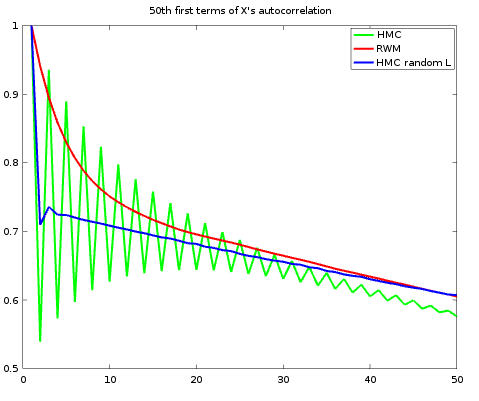
\includegraphics[width=.8\textwidth]{figs/gm_autocor.png}
  \end{center}  
\end{frame}

\subsection{Bayesian Lasso}
\begin{frame}
  \frametitle{Bayesian Lasso}
\begin{itemize}
\item $U(x) = \norm{Ax - b}_2^2 + \lambda \norm{x}_1$ non différentiable.
\item On considère la sous-différentielle $(A + A^\top) x + \lambda \sign(x)$ 
\end{itemize}
\end{frame}
\begin{frame}
  \frametitle{Bayesian Lasso : trajectoires}
\begin{center}
    \includemovie[autoplay, poster]{\textwidth}{.9\textheight}{figs/bl.mp4}
  \end{center}  
\end{frame}

\begin{frame}
  \frametitle{Bayesian Lasso : autocorrelations}
\begin{center}
      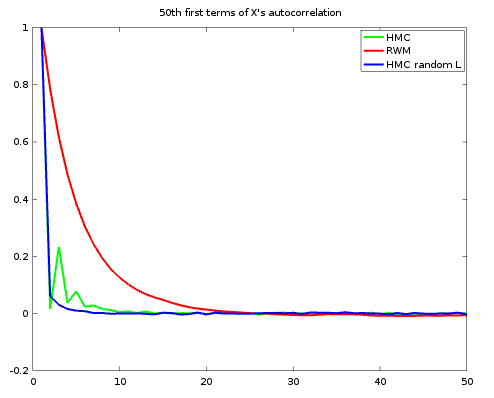
\includegraphics[width=.8\textwidth]{figs/bl_autocor.png}
  \end{center}  
\end{frame}

\begin{frame}
  \frametitle{Bayesian Lasso : loin du mode}
\begin{center}
    \includemovie[autoplay, poster]{\textwidth}{.9\textheight}{figs/bl_far.mp4}
  \end{center}  
\end{frame}

\section{Conclusion}
\begin{frame}
  \frametitle{Conclusion}
  \begin{itemize}
  \item Le HMC construit une chaîne de Markov de loi invariante la loi cible dans les cas idéal et approché.
  \item Certaines hypothèses sont nécessaires pour avoir l'invariance (problème dans le Bayesian Lasso).
  \item Prendre $L$ aléatoire semble améliorer la stationnarité
  \end{itemize}
\end{frame}
\end{document}


